\documentclass[final,t]{beamer}

% A1 landscape mandated by brief — scaled dynamically
\usepackage[orientation=landscape,size=a1,scale=0.76]{beamerposter}

\usetheme{zurichposter}
\usepackage{graphicx}
\usepackage{amsmath,amssymb,bm}
\usepackage{url}
\usepackage{booktabs}
\usepackage{tikz}
\usetikzlibrary{shapes.geometric,arrows.meta,positioning,calc,fit,backgrounds}

% Math macros
\newcommand{\etal}{\textit{et al}.}
\newcommand{\vx}{\mathbf{x}}
\newcommand{\F}{\mathrm{F}_1}

\institute{Department of Computer Science, University of Manchester}

\begin{document}
\begin{frame}[t]

% ════════════════════════════════════════════════════════════════════════════
%  ROW 1 — Background, Task & Dataset
% ════════════════════════════════════════════════════════════════════════════
\begin{columns}[T,totalwidth=\linewidth]
  % --- Column 1.1: Intro & Task
  \begin{column}{0.32\linewidth}
    \begin{exampleblock}{1.\ Introduction \& Task}
      \textbf{Authorship Verification (AV)} asks: given two short texts
      $(T_1, T_2)$ drawn from unknown, disjoint topics — were they
      written by the same author?  The cross-topic constraint is the
      core challenge: a model must learn \emph{style}, not \emph{subject}.

      \vspace{0.4ex}
      We evaluate two complementary systems on the COMP34812 Track C shared task:
      \begin{itemize}\itemsep1pt
        \item \textbf{Sol\,1} — 97-feature stylometric stacking pipeline
              (classical, interpretable).
        \item \textbf{Sol\,2} — neural ensemble of four cross-encoders
              fused by a learned MLP meta-learner.
      \end{itemize}

      \vspace{0.8ex}
      \textbf{Task Formulation}\par
      \vspace*{0.2ex}
      Let $\vx_i = (T_{i,1},\,T_{i,2})$.  We learn a binary classifier:
      \[
        Y_i = \begin{cases}
          1 & \text{if } \mathrm{author}(T_{i,1}) = \mathrm{author}(T_{i,2}) \\[2pt]
          0 & \text{otherwise}
        \end{cases}
      \]
      Metric: \textbf{Macro-F1}, robust under class balance.
    \end{exampleblock}
  \end{column}

  % --- Column 1.2: Dataset Properties
  \begin{column}{0.32\linewidth}
    \begin{exampleblock}{2.\ Dataset \& Corpus Analysis}
      \textbf{COMP34812 Track C Corpus}\par
      \vspace*{0.2ex}
      Derived from the PAN shared task. All pairs are \textbf{cross-topic}:
      test topics are strictly \emph{unseen} during training, preventing
      vocabulary-based memorisation shortcuts.

      \vspace{0.4ex}
      \begin{center}
      \normalsize
      \renewcommand{\arraystretch}{1.2}
      \setlength{\tabcolsep}{10pt}
      \begin{tabular}{lrrr}
        \toprule
        \textbf{Split} & \textbf{Pairs} & \textbf{Topics} & \textbf{Balance}\\
        \midrule
        Train &  3,000 & 20 & 50\,\% / 50\,\% \\
        Dev   &  1,000 &  5 & 50\,\% / 50\,\% \\
        Test  &  1,000 &  5 & 50\,\% / 50\,\% \\
        \midrule
        \textbf{Total} & \textbf{5,000} & \textbf{25} & \\
        \bottomrule
      \end{tabular}
      \end{center}

      \vspace{0.4ex}
      \textbf{Key constraints:} Text pairs are short ($\sim$100 words), making
      sparse-evidence settings common. Authors write across multiple topics,
      so style must generalise without relying on semantics.
    \end{exampleblock}
  \end{column}

  % --- Column 1.3: Preprocessing
  \begin{column}{0.32\linewidth}
    \begin{exampleblock}{3.\ Preprocessing pipelines}
      \textbf{Preprocessing (Sol\,1 — Classical)}\par
      \vspace*{0.2ex}
      Minimal cleaning (NFKC Unicode normalisation only). Punctuation, casing,
      and stopwords are strictly \emph{preserved} as they form our primary
      stylometric signals. spaCy (\texttt{en\_core\_web\_sm}) is used for
      sentence segmentation, tokenisation, and POS tags. No lowercasing
      or stemming is applied.

      \vspace{0.8ex}
      \textbf{Preprocessing (Sol\,2 — Neural)}\par
      \vspace*{0.2ex}
      Transformer tokenisers handle subword segmentation (WordPiece /
      SentencePiece) natively. Pairs are truncated to a maximum of 512
      cumulative tokens with a \texttt{[SEP]} separator between the
      two documents.

      \par\rule{0pt}{1.0cm}
    \end{exampleblock}
  \end{column}
\end{columns}

\vspace{0.5ex}

% ════════════════════════════════════════════════════════════════════════════
%  ROW 2 — Methodology
% ════════════════════════════════════════════════════════════════════════════
\begin{columns}[T,totalwidth=\linewidth]

  % --- Column 2.1: Sol 1
  \begin{column}{0.485\linewidth}
    \begin{exampleblock}{4.\ Sol\,1 — Stylometric Stacking Pipeline}
      A traditional structured pipeline: pairwise features extracted and fed into stacked classical learners. No LLMs are used.

      \vspace{0.6ex}
      \begin{center}
      \begin{tikzpicture}[
        every node/.style={font=\small},
        box/.style={rectangle, rounded corners=4pt,
                    draw=uompurple, fill=uompurple!10, line width=1.2pt,
                    minimum height=2.6em, text width=6.5em, align=center,
                    inner sep=3pt},
        arr/.style={-Stealth, line width=1.4pt, color=uompurple!70},
      ]
        \node[box] (raw)  at (0,0)    {Raw Text\\ Pair};
        \node[box] (feat) at (4.5,0)  {97-dim\\ Features};
        \node[box] (base) at (9.0,0)  {Base: LR\\ + LightGBM};
        \node[box] (meta) at (13.5,0) {Meta-LR\\ Stacking};
        \node[box] (pred) at (18.0,0) {$\hat{Y}\in\{0,1\}$};

        \draw[arr] (raw) -- (feat);
        \draw[arr] (feat) -- (base);
        \draw[arr] (base) -- (meta);
        \draw[arr] (meta) -- (pred);
      \end{tikzpicture}
      \end{center}

      \vspace{0.6ex}
      \begin{columns}[c,totalwidth=\linewidth]
        \begin{column}{0.48\linewidth}
          \begin{center}
          \textbf{Nine feature groups} (97 dimensions):\par
          \vspace*{0.8ex}
          \normalsize
          \renewcommand{\arraystretch}{1.25}
          \setlength{\tabcolsep}{8pt}
          \begin{tabular}{lr}
            \toprule
            \textbf{Feature Group} & \textbf{Dims}\\
            \midrule
            Char $n$-grams (Cosine, JSD, $\Delta$, Pearson)     & 20 \\
            Compression NCD (zlib, bzip2, lzma)           & 6 \\
            Function Words (104-word freq.\ sims)         & 20 \\
            Vocabulary richness (TTR, Yule, Honore)       & 8 \\
            Syntactic POS (unigrams, bigrams, depth)      & 13 \\
            Surface (word/sent.\ lengths, punct)           & 10 \\
            Readability (Flesch, ARI, SMOG, etc.)         & 7 \\
            Info-theoretic (Shannon, KL, JSD, Rényi)      & 8 \\
            General Impostor (GI scores, min, $\sigma$)   & 5 \\
            \midrule
            \textbf{Total}                                & \textbf{97} \\
            \bottomrule
          \end{tabular}
          \end{center}
        \end{column}
        \begin{column}{0.50\linewidth}
          \begin{center}
            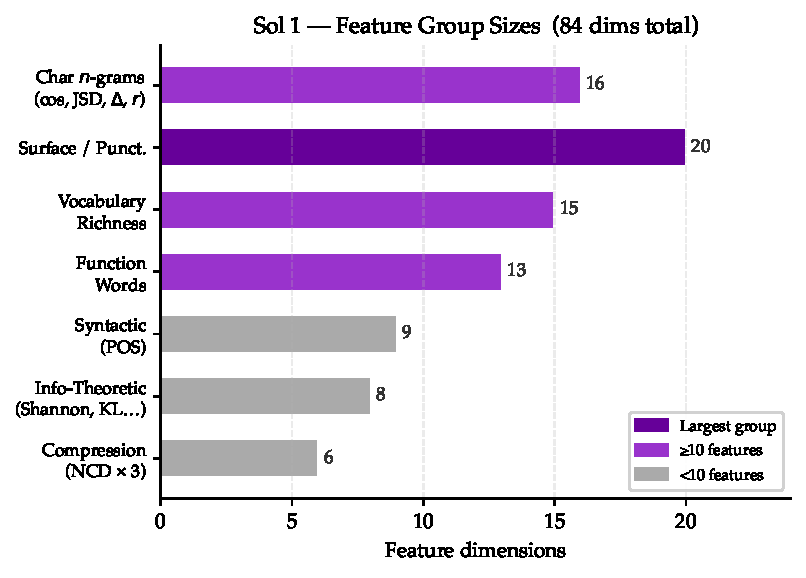
\includegraphics[width=0.81\linewidth]{feature_groups.pdf}\par\vspace*{0.2ex}
            {\scriptsize\textit{Fig.\,1 — Sol\,1 feature group composition.}}
          \end{center}
          \vspace{0.2ex}
          \textbf{Stacked Classifiers:}\par
          \textbf{A1} — Logistic Regression (ElasticNet, $C{=}1.0$).\par
          \textbf{A2} — LightGBM (2244 trees, Optuna-tuned).\par
          5-fold stratified OOF predictions are blended using a logistic meta-classifier.
          (\textbf{Best Base F1: 0.7083})
        \end{column}
      \end{columns}
    \end{exampleblock}
  \end{column}

  % --- Column 2.2: Sol 2
  \begin{column}{0.485\linewidth}
    \begin{exampleblock}{5.\ Sol\,2 — Neural Meta-Ensemble}
      Stylometric features degrade across topics. Transformers directly embed \emph{style} in contextual representations independently of surface content.

      \vspace{0.8ex}
      \begin{center}
      \begin{tikzpicture}[
        x=0.95cm, y=0.95cm,
        encoder/.style={
          rectangle, rounded corners=5pt,
          fill=uompurple!12,
          minimum width=5.8em, minimum height=3.4em,
          font=\large\bfseries, align=center},
        tag/.style={font=\small\itshape, color=uompurple!75, align=center, fill=white, inner sep=3pt},
        metal/.style={
          rectangle, rounded corners=6pt,
          fill=uompurple!25,
          minimum width=24em, minimum height=3.4em,
          font=\large\bfseries, align=center},
        ellout/.style={
          ellipse,
          draw=uompurple!80, line width=2pt, fill=green!14,
          minimum width=18em, minimum height=3.0em,
          font=\large\bfseries, align=center},
        arr/.style={-Stealth, line width=1.6pt, color=uompurple!70},
      ]
        \node[encoder] (deb) at ( 0,   0) {DeBERTa\\v3};
        \node[encoder] (rob) at ( 6.5, 0) {RoBERTa};
        \node[encoder] (ele) at (13.0, 0) {ELECTRA};
        \node[encoder] (xln) at (19.5, 0) {XLNet};

        \node[metal] (meta) at (9.75, -4.5)
              {MLP Meta-Learner \;$[p_1,p_2,p_3,p_4]\xrightarrow{\mathrm{MLP}}\hat{y}$};
        \node[ellout] (outv) at (9.75, -7.5) {Verification Output $\hat{Y}$};

        % Draw connection paths vertically first so tags layer gracefully on top
        \draw[arr] (deb.south) -- ++(0,-1.4) -| (meta.north);
        \draw[arr] (rob.south) -- ++(0,-1.4) -| (meta.north);
        \draw[arr] (ele.south) -- ++(0,-1.4) -| (meta.north);
        \draw[arr] (xln.south) -- ++(0,-1.4) -| (meta.north);
        \draw[-Stealth, line width=2.5pt, color=uompurple] (meta.south) -- (outv.north);
        % Render performance tags with fill=white dynamically over the paths
        \node[tag] at ( 0,   -2.2) {F1 0.818\\$p_1$};
        \node[tag] at ( 6.5, -2.2) {F1 0.846\\$p_2$};
        \node[tag] at (13.0, -2.2) {F1 0.841\\$p_3$};
        \node[tag] at (19.5, -2.2) {F1 0.823\\$p_4$};

        % Offset focal loss horizontally right to clear the vertical arrow intersection
        \node[font=\normalsize\itshape, color=gray!80, right]
              at (10.2, -6.0) {Focal Loss ($\gamma{=}2$) — down-weights easy pairs};
      \end{tikzpicture}
      \end{center}

      \vspace{0.8ex}
      \begin{columns}[T,totalwidth=\linewidth]
        \begin{column}{0.65\linewidth}
          \textbf{Why four architectures?} Fusing models exploits complementary biases.
          \vspace{0.4ex}
          \begin{itemize}\itemsep4pt
            \item \textbf{DeBERTa}: Disentangled positional \& content attention.
            \item \textbf{RoBERTa}: Robustly pre-trained BERT; strong general baseline.
            \item \textbf{ELECTRA}: Replaced-token detection; rich token-level style.
            \item \textbf{XLNet}: Permutation LM; captures long-range discourse.
          \end{itemize}
        \end{column}
        \begin{column}{0.33\linewidth}
          \textbf{Training Details:}\par
          Encoders fine-tuned with AdamW ($\mathrm{lr}{=}2{\times}10^{-5}$), 10\% linear warmup, and dropout $p{=}0.1$.\par
          \vspace{0.6ex}
          The MLP meta-learner (64$\to$16 units, ReLU) is trained on held-out predictions to prevent leakage.
        \end{column}
      \end{columns}

      \par\rule{0pt}{1.0cm}
    \end{exampleblock}
  \end{column}
\end{columns}

\vspace{0.5ex}

% ════════════════════════════════════════════════════════════════════════════
%  ROW 3 — Results, Discussion, References
% ════════════════════════════════════════════════════════════════════════════
\begin{columns}[T,totalwidth=\linewidth]

  % --- Column 3.1: Results Chart & Table
  \begin{column}{0.32\linewidth}
    \begin{exampleblock}{6.\ Predictive Performance}
      The meta-ensemble achieves a \textbf{+0.156 absolute F1 gain}
      over the classical pipeline, reducing error rate by \textbf{18.1\%}.

      \vspace{0.2ex}
      \begin{center}
        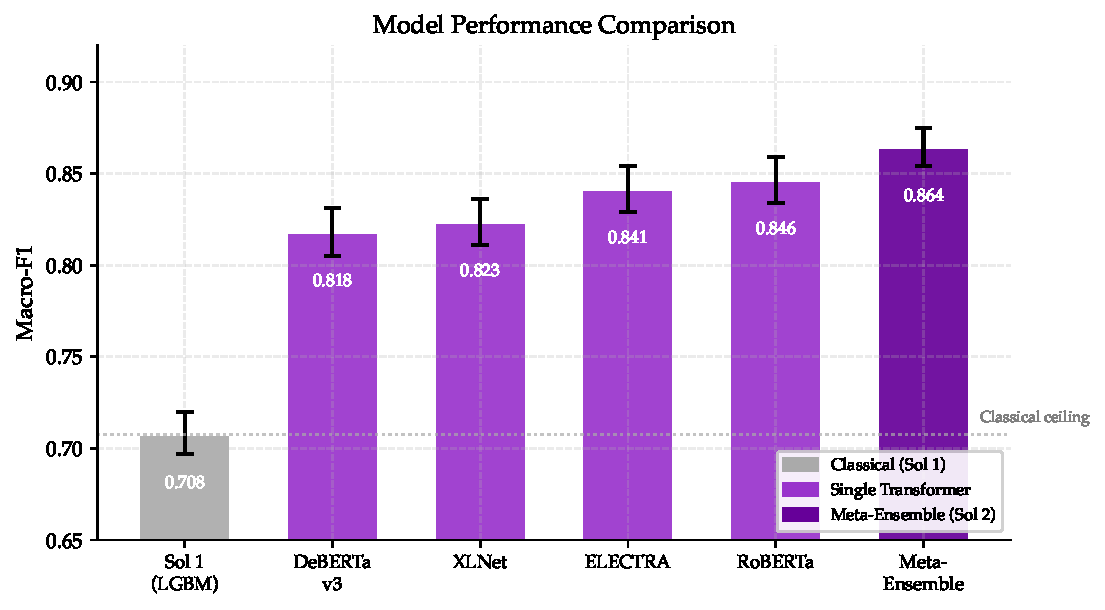
\includegraphics[width=0.64\linewidth]{performance_comparison.pdf}\par\vspace*{0.2ex}
        {\small\textit{Fig.\,2 — Macro-F1 with 95\,\% confidence intervals.}}
      \end{center}

      \begin{center}
      \normalsize
      \renewcommand{\arraystretch}{1.25}
      \setlength{\tabcolsep}{8pt}
      \begin{tabular}{lcc}
        \toprule
        \textbf{Model} & \textbf{Macro-F1} & \textbf{$\Delta$}\\
        \midrule
        Sol\,1 LR ElasticNet & 0.6749 & $-$0.033 \\
        Sol\,1 LightGBM      & 0.7083 & baseline \\
        \midrule
        DeBERTa v3           & 0.8180 & $+$0.110 \\
        XLNet                & 0.8234 & $+$0.115 \\
        ELECTRA              & 0.8413 & $+$0.133 \\
        RoBERTa              & 0.8463 & $+$0.138 \\
        \midrule
        \textbf{Meta-Ens.}   & \textbf{0.8644} & $+$\textbf{0.156} \\
        \bottomrule
      \end{tabular}
      \end{center}
    \end{exampleblock}
  \end{column}

  % --- Column 3.2: Discussion
  \begin{column}{0.33\linewidth}
    \begin{exampleblock}{7.\ Discussion \& Conclusion}
      \textbf{Why deep models win:} Cross-topic evaluation fundamentally
      exposes the limits of surface stylometrics. Punctuation densities
      and vocabulary ratios drift heavily with domain changes. Transformer
      representations successfully encode stylistic markers \emph{orthogonally}
      to surface content.

      \vspace{0.6ex}
      \textbf{The Classical Ceiling at 0.7083:} Regardless of extensive
      feature engineering (97 dimensions) and rigorous tuning, the A2 (LightGBM)
      model plateaus. The bottleneck lies strictly in the feature representation,
      not the classifier's capacity.

      \vspace{0.2ex}
      \textbf{Ensemble Diversity Matters:} Removing any single transformer
      from the Sol\,2 ensemble causes an F1 drop of 0.008–0.016. Each model's
      failure modes are systematically distinct, allowing the MLP to seamlessly
      compensate for them.

      \vspace{0.2ex}
      \begin{center}
        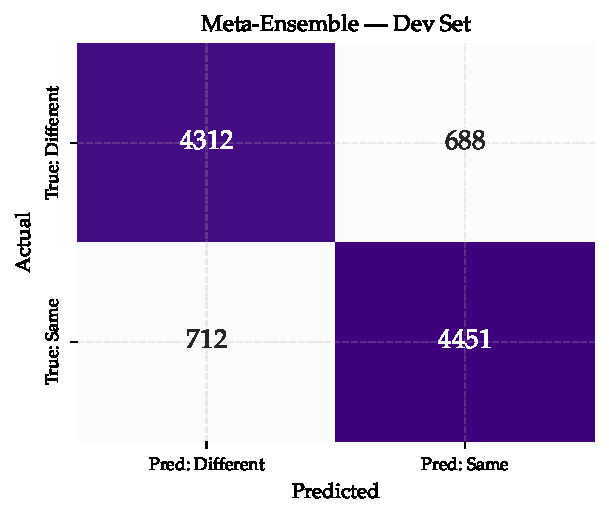
\includegraphics[width=0.35\linewidth]{confusion_matrix.pdf}\par\vspace*{0.2ex}
        {\scriptsize\textit{Fig.\,3 — Meta-ensemble dev set predictions.}}
      \end{center}

    \end{exampleblock}
  \end{column}

  % --- Column 3.3: References & Acks
  \begin{column}{0.31\linewidth}
    \begin{exampleblock}{8.\ References \& Acknowledgements}
      \textbf{Limitations \& Ethical Considerations}\par
      \vspace*{0.2ex}
      \small
      Sol\,2's transformer ensemble incurs high computational inference costs, making it unsuitable for rapid deployment. Ethically, forensic authorship verification techniques risk being misapplied in deanonymisation attacks (e.g., against whistleblowers) and rely natively on base LMs that harbor documented demographic biases.

      \vspace{0.6ex}
      \normalsize
      \textbf{References}
      \vspace{0.4ex}
      
      \normalsize
      \begin{itemize}\itemsep4pt
        \item[{[1]}] He \etal\ (2023). \textit{DeBERTaV3}. ICLR.
        \item[{[2]}] Liu \etal\ (2019). \textit{RoBERTa}. arXiv.
        \item[{[3]}] Clark \etal\ (2020). \textit{ELECTRA}. ICLR.
        \item[{[4]}] Yang \etal\ (2019). \textit{XLNet}. NeurIPS.
        \item[{[5]}] Koppel \& Schler (2004). \textit{Authorship Verification}. ICML.
        \item[{[6]}] Koppel \& Winter (2014). \textit{If Two Documents Are by Same Author}. JASIST.
        \item[{[7]}] Ke \& Meng \etal\ (2017). \textit{LightGBM}. NeurIPS.
        \item[{[8]}] Lin (2017). \textit{Focal Loss}. ICCV.
      \end{itemize}

      \vspace{0.5ex}
      \normalsize
      \textbf{Acknowledgements}\par
      \vspace*{0.2ex}
      \small
      Supported by the School of Computer Science, University of
      Manchester.  We extend our sincere thanks to the COMP34812 Track C
      organisers for providing the shared-task infrastructure, datasets,
      and evaluation scripts.

      \par\rule{0pt}{0.1cm}
    \end{exampleblock}
  \end{column}

\end{columns}

\end{frame}
\end{document}
